\documentclass[letterpaper]{article}

\usepackage[margin=1in]{geometry}
\usepackage{bytefield}
\usepackage{graphicx}
\usepackage{parskip}
\usepackage{pdfpages}
\usepackage{fontspec}
\usepackage{xcolor}

\setmonofont{Inconsolata}

\newsavebox{\arithbox}
\newsavebox{\loadbox}
\newsavebox{\branchbox}
\newsavebox{\miscbox}
\newsavebox{\regbox}

\newcommand\bitwidth{1.25em}
\newcommand\instskip{0.5em}
\newcommand\instwidth{0.72\linewidth}
%\newcommand\instgap{\vspace{1em}\hrule\vspace{1em}}
\newcommand\instgap{\vspace{0.4em}\hrule\vspace{0.25em}}
%\newcommand\instgap{\rule{\linewidth}{0.6pt}}
%\newcommand\instgap{\hrule}

% don't use -- since it looks like a minus sign
\renewcommand{\labelitemii}{\labelitemi}

\newif\ifbaby
% Set to true to get a "baby" reference sheet with a simpler datapath. Set to
% false to get a full reference sheet with TRAPs and I/O.
\babytrue
%\babyfalse

\newif\ifc
% Set to true to get a C ref sheet with a memory map focused on compiling C to assembly.
% Set false to get a memory map with interrupts/MMIO
\ctrue
%\cfalse

\begin{document}
    \centering
    \section*{LC-3 Instruction Encodings}

%\subsection*{Arithmetic/Logical Instructions}
%\vspace{1em}
\begin{lrbox}{\arithbox}
    \begin{bytefield}[bitwidth=\bitwidth]{20}
        \bitheader[endianness=big]{0-15} \\
        % add register
        \bitbox[r]{4}{\hfill\textbf{ADD}${}^\dagger$\:\:}
        & \bitbox[ltb]{1}{0}
        & \bitbox[tb]{1}{0}
        & \bitbox[tb]{1}{0}
        & \bitbox[tbr]{1}{1}
        & \bitbox[ltbr]{3}{DR}
        & \bitbox[ltbr]{3}{SR1}
        & \bitbox[ltb]{1}{0}
        & \bitbox[tb]{1}{0}
        & \bitbox[tbr]{1}{0}
        & \bitbox[ltbr]{3}{SR2}
        \\[\instskip]
        % add immediate
        \bitbox[r]{4}{\hfill\textbf{ADD}${}^\dagger$\:\:}
        & \bitbox[ltb]{1}{0}
        & \bitbox[tb]{1}{0}
        & \bitbox[tb]{1}{0}
        & \bitbox[tbr]{1}{1}
        & \bitbox[ltbr]{3}{DR}
        & \bitbox[ltbr]{3}{SR1}
        & \bitbox[ltbr]{1}{1}
        & \bitbox[ltbr]{5}{imm5}
        \\[\instskip]
        % and register
        \bitbox[r]{4}{\hfill\textbf{AND}${}^\dagger$\:\:}
        & \bitbox[ltb]{1}{0}
        & \bitbox[tb]{1}{1}
        & \bitbox[tb]{1}{0}
        & \bitbox[tbr]{1}{1}
        & \bitbox[ltbr]{3}{DR}
        & \bitbox[ltbr]{3}{SR1}
        & \bitbox[ltb]{1}{0}
        & \bitbox[tb]{1}{0}
        & \bitbox[tbr]{1}{0}
        & \bitbox[ltbr]{3}{SR2}
        \\[\instskip]
        % and immediate
        \bitbox[r]{4}{\hfill\textbf{AND}${}^\dagger$\:\:}
        & \bitbox[ltb]{1}{0}
        & \bitbox[tb]{1}{1}
        & \bitbox[tb]{1}{0}
        & \bitbox[tbr]{1}{1}
        & \bitbox[ltbr]{3}{DR}
        & \bitbox[ltbr]{3}{SR1}
        & \bitbox[ltbr]{1}{1}
        & \bitbox[ltbr]{5}{imm5}
        \\[\instskip]
        % not
        \bitbox[r]{4}{\hfill\textbf{NOT}${}^\dagger$\:\:}
        & \bitbox[ltb]{1}{1}
        & \bitbox[tb]{1}{0}
        & \bitbox[tb]{1}{0}
        & \bitbox[tbr]{1}{1}
        & \bitbox[ltbr]{3}{DR}
        & \bitbox[ltbr]{3}{SR}
        & \bitbox[ltb]{1}{1}
        & \bitbox[tb]{1}{1}
        & \bitbox[tb]{1}{1}
        & \bitbox[tb]{1}{1}
        & \bitbox[tb]{1}{1}
        & \bitbox[tbr]{1}{1}
    \end{bytefield}%
\end{lrbox}
\raisebox{.5\height}{\rotatebox{90}{\large \textbf{Arith./Logic}}}
\resizebox*{\instwidth}{!}{\usebox{\arithbox}}

\instgap{}

%\subsection*{Load/Store Instructions}
%\vspace{1em}
\begin{lrbox}{\loadbox}
    \begin{bytefield}[bitwidth=\bitwidth]{20}
        \bitheader[endianness=big]{0-15} \\
        % ld
        \bitbox[r]{4}{\hfill\textbf{LD}${}^\dagger$\:\:}
        & \bitbox[ltb]{1}{0}
        & \bitbox[tb]{1}{0}
        & \bitbox[tb]{1}{1}
        & \bitbox[tbr]{1}{0}
        & \bitbox[ltbr]{3}{DR}
        & \bitbox[ltbr]{9}{PCoffset9}
        \\[\instskip]
        % st
        \bitbox[r]{4}{\hfill\textbf{ST}\:\:}
        & \bitbox[ltb]{1}{0}
        & \bitbox[tb]{1}{0}
        & \bitbox[tb]{1}{1}
        & \bitbox[tbr]{1}{1}
        & \bitbox[ltbr]{3}{SR}
        & \bitbox[ltbr]{9}{PCoffset9}
        \\[\instskip]
        % ldi
        \bitbox[r]{4}{\hfill\textbf{LDI}${}^\dagger$\:\:}
        & \bitbox[ltb]{1}{1}
        & \bitbox[tb]{1}{0}
        & \bitbox[tb]{1}{1}
        & \bitbox[tbr]{1}{0}
        & \bitbox[ltbr]{3}{DR}
        & \bitbox[ltbr]{9}{PCoffset9}
        \\[\instskip]
        % sti
        \bitbox[r]{4}{\hfill\textbf{STI}\:\:}
        & \bitbox[ltb]{1}{1}
        & \bitbox[tb]{1}{0}
        & \bitbox[tb]{1}{1}
        & \bitbox[tbr]{1}{1}
        & \bitbox[ltbr]{3}{SR}
        & \bitbox[ltbr]{9}{PCoffset9}
        \\[\instskip]
        % ldr
        \bitbox[r]{4}{\hfill\textbf{LDR}${}^\dagger$\:\:}
        & \bitbox[ltb]{1}{0}
        & \bitbox[tb]{1}{1}
        & \bitbox[tb]{1}{1}
        & \bitbox[tbr]{1}{0}
        & \bitbox[ltbr]{3}{DR}
        & \bitbox[ltbr]{3}{BaseR}
        & \bitbox[ltbr]{6}{offset6}
        \\[\instskip]
        % str
        \bitbox[r]{4}{\hfill\textbf{STR}\:\:}
        & \bitbox[ltb]{1}{0}
        & \bitbox[tb]{1}{1}
        & \bitbox[tb]{1}{1}
        & \bitbox[tbr]{1}{1}
        & \bitbox[ltbr]{3}{SR}
        & \bitbox[ltbr]{3}{BaseR}
        & \bitbox[ltbr]{6}{offset6}
        %\\[\instskip]
    \end{bytefield}%
\end{lrbox}
\raisebox{.85\height}{\rotatebox{90}{\large \textbf{Load/Store}}}
\resizebox*{\instwidth}{!}{\usebox{\loadbox}}

\instgap{}

%\subsection*{Branch Instructions}
%\vspace{1em}
\begin{lrbox}{\branchbox}
    \begin{bytefield}[bitwidth=\bitwidth]{20}
        \bitheader[endianness=big]{0-15} \\
        % jmp
        \bitbox[r]{4}{\hfill\textbf{JMP}\:\:}
        & \bitbox[ltb]{1}{1}
        & \bitbox[tb]{1}{1}
        & \bitbox[tb]{1}{0}
        & \bitbox[tbr]{1}{0}
        & \bitbox[ltb]{1}{0}
        & \bitbox[tb]{1}{0}
        & \bitbox[tbr]{1}{0}
        & \bitbox[ltbr]{3}{BaseR}
        & \bitbox[ltb]{1}{0}
        & \bitbox[tb]{1}{0}
        & \bitbox[tb]{1}{0}
        & \bitbox[tb]{1}{0}
        & \bitbox[tb]{1}{0}
        & \bitbox[tbr]{1}{0}
        \\[\instskip]
        % br
        \bitbox[r]{4}{\hfill\textbf{BR}\:\:}
        & \bitbox[ltb]{1}{0}
        & \bitbox[tb]{1}{0}
        & \bitbox[tb]{1}{0}
        & \bitbox[tbr]{1}{0}
        & \bitbox[ltbr]{1}{cn}
        & \bitbox[ltbr]{1}{cz}
        & \bitbox[ltbr]{1}{\vspace{1.5pt}cp}
        & \bitbox[ltbr]{9}{PCoffset9}
        \\[\instskip]
        % jsrr
        \bitbox[r]{4}{\hfill\textbf{JSRR}\:\:}
        & \bitbox[ltb]{1}{0}
        & \bitbox[tb]{1}{1}
        & \bitbox[tb]{1}{0}
        & \bitbox[tbr]{1}{0}
        & \bitbox[ltb]{1}{0}
        & \bitbox[tb]{1}{0}
        & \bitbox[tbr]{1}{0}
        & \bitbox[ltbr]{3}{BaseR}
        & \bitbox[ltb]{1}{0}
        & \bitbox[tb]{1}{0}
        & \bitbox[tb]{1}{0}
        & \bitbox[tb]{1}{0}
        & \bitbox[tb]{1}{0}
        & \bitbox[tbr]{1}{0}
        \\[\instskip]
        % jsr
        \bitbox[r]{4}{\hfill\textbf{JSR}\:\:}
        & \bitbox[ltb]{1}{0}
        & \bitbox[tb]{1}{1}
        & \bitbox[tb]{1}{0}
        & \bitbox[tbr]{1}{0}
        & \bitbox[ltbr]{1}{1}
        & \bitbox[ltbr]{11}{PCoffset11}
    \end{bytefield}%
\end{lrbox}
\raisebox{0.95\height}{\rotatebox{90}{\large \textbf{Branch}}}
\resizebox*{\instwidth}{!}{\usebox{\branchbox}}

\instgap{}

%\subsection*{Miscellaneous Instructions}
%\vspace{1em}
\begin{lrbox}{\miscbox}
    \begin{bytefield}[bitwidth=\bitwidth]{20}
        \bitheader[endianness=big]{0-15} \\
        % lea
        \bitbox[r]{4}{\hfill\textbf{LEA}\:\:}
        & \bitbox[ltb]{1}{1}
        & \bitbox[tb]{1}{1}
        & \bitbox[tb]{1}{1}
        & \bitbox[tbr]{1}{0}
        & \bitbox[ltbr]{3}{DR}
        & \bitbox[ltbr]{9}{PCoffset9}
        \\[\instskip]
        % trap
        \bitbox[r]{4}{\hfill\textbf{TRAP}\:\:}
        & \bitbox[ltb]{1}{1}
        & \bitbox[tb]{1}{1}
        & \bitbox[tb]{1}{1}
        & \bitbox[tbr]{1}{1}
        & \bitbox[ltb]{1}{0}
        & \bitbox[tb]{1}{0}
        & \bitbox[tb]{1}{0}
        & \bitbox[tbr]{1}{0}
        & \bitbox[ltbr]{8}{trapvect8}
        \\[\instskip]
        % rti
        \bitbox[r]{4}{\hfill\textbf{RTI}\:\:}
        & \bitbox[ltb]{1}{1}
        & \bitbox[tb]{1}{0}
        & \bitbox[tb]{1}{0}
        & \bitbox[tbr]{1}{0}
        & \bitbox[ltb]{1}{0}
        & \bitbox[tb]{1}{0}
        & \bitbox[tb]{1}{0}
        & \bitbox[tb]{1}{0}
        & \bitbox[tb]{1}{0}
        & \bitbox[tb]{1}{0}
        & \bitbox[tb]{1}{0}
        & \bitbox[tb]{1}{0}
        & \bitbox[tb]{1}{0}
        & \bitbox[tb]{1}{0}
        & \bitbox[tb]{1}{0}
        & \bitbox[tbr]{1}{0}
        \\[\instskip]
        % illegal
        \bitbox[r]{4}{\hfill\textit{illegal}\:\:}
        & \bitbox[ltb]{1}{1}
        & \bitbox[tb]{1}{1}
        & \bitbox[tb]{1}{0}
        & \bitbox[tbr]{1}{1}
        & \bitbox[ltb]{1}{x}
        & \bitbox[tb]{1}{x}
        & \bitbox[tb]{1}{x}
        & \bitbox[tb]{1}{x}
        & \bitbox[tb]{1}{x}
        & \bitbox[tb]{1}{x}
        & \bitbox[tb]{1}{x}
        & \bitbox[tb]{1}{x}
        & \bitbox[tb]{1}{x}
        & \bitbox[tb]{1}{x}
        & \bitbox[tb]{1}{x}
        & \bitbox[tbr]{1}{x}
    \end{bytefield}%
\end{lrbox}
\raisebox{1.55\height}{\rotatebox{90}{\large \textbf{Misc.}}}
\resizebox*{\instwidth}{!}{\usebox{\miscbox}}

\instgap{}

{\large $\dagger$ \textit{Updates condition code (CC)}}


    \ifbaby
        \ifc
            \newpage
\section*{LC-3 MMIO Registers}

\begin{lrbox}{\regbox}
    \begin{bytefield}[bitwidth=\bitwidth]{23}
        %\bitbox[]{4}{\textbf{Address}\hfill} \\
        \bitheader[endianness=big]{0-15} \\
        \bitbox[]{3}{\texttt{0xFE00}\hfill}
        & \bitbox[r]{4}{\hfill\textbf{KBSR}\:\:}
        & \bitbox[ltb]{1}{\rotatebox{90}{\footnotesize Rdy}}
        & \bitbox[ltbr]{15}{\footnotesize\color{gray}\textit{(undefined)}}
        \\[\instskip]
        \bitbox[]{3}{\texttt{0xFE02}\hfill}
        & \bitbox[r]{4}{\hfill\textbf{KBDR}\:\:}
        & \bitbox[ltb]{1}{0}
        & \bitbox[tb]{1}{0}
        & \bitbox[tb]{1}{0}
        & \bitbox[tb]{1}{0}
        & \bitbox[tb]{1}{0}
        & \bitbox[tb]{1}{0}
        & \bitbox[tb]{1}{0}
        & \bitbox[tb]{1}{0}
        & \bitbox[ltbr]{8}{ASCII code}
        \\[\instskip]
        \bitbox[]{3}{\texttt{0xFE04}\hfill}
        & \bitbox[r]{4}{\hfill\textbf{DSR}\:\:}
        & \bitbox[ltb]{1}{\rotatebox{90}{\footnotesize Rdy}}
        & \bitbox[ltbr]{15}{\footnotesize\color{gray}\textit{(undefined)}}
        \\[\instskip]
        \bitbox[]{3}{\texttt{0xFE06}\hfill}
        & \bitbox[r]{4}{\hfill\textbf{DDR}\:\:}
        & \bitbox[ltb]{1}{0}
        & \bitbox[tb]{1}{0}
        & \bitbox[tb]{1}{0}
        & \bitbox[tb]{1}{0}
        & \bitbox[tb]{1}{0}
        & \bitbox[tb]{1}{0}
        & \bitbox[tb]{1}{0}
        & \bitbox[tb]{1}{0}
        & \bitbox[ltbr]{8}{ASCII code}
        \\[\instskip]
        \bitbox[]{3}{\texttt{0xFFFC}\hfill}
        & \bitbox[r]{4}{\hfill\textbf{PSR}\:\:}
        & \bitbox[ltbr]{1}{\rotatebox{90}{\footnotesize Priv}}
        & \bitbox[ltbr]{4}{\footnotesize\color{gray}\textit{(undefined)}}
        & \bitbox[ltbr]{3}{PRIO}
        & \bitbox[ltbr]{5}{\footnotesize\color{gray}\textit{(undefined)}}
        & \bitbox[ltbr]{1}{N}
        & \bitbox[ltbr]{1}{Z}
        & \bitbox[ltbr]{1}{P}
        %\\[\instskip]
    \end{bytefield}%
\end{lrbox}
%\raisebox{.5\height}{\rotatebox{90}{\large \textbf{Arith./Logic}}}
\resizebox*{0.85\linewidth}{!}{\usebox{\regbox}}

\section*{LC-3 Trap Vectors}
\begin{minipage}{11em}
\Large
\begin{itemize}
    \item \texttt{0x20} $\rightarrow$ \texttt{GETC}
    \item \texttt{0x21} $\rightarrow$ \texttt{PUTC}
    \item \texttt{0x22} $\rightarrow$ \texttt{PUTS}
    \item \texttt{0x25} $\rightarrow$ \texttt{HALT}
\end{itemize}
\end{minipage}

\section*{LC-3 Memory Map}
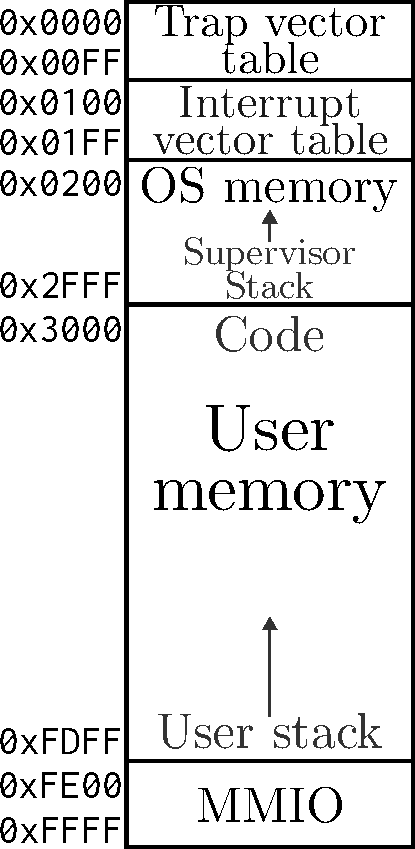
\includegraphics[width=0.33\linewidth]{figs/lc3-memory-map}

        \fi
    \else
        \newpage
\section*{LC-3 MMIO Registers}

\begin{lrbox}{\regbox}
    \begin{bytefield}[bitwidth=\bitwidth]{23}
        %\bitbox[]{4}{\textbf{Address}\hfill} \\
        \bitheader[endianness=big]{0-15} \\
        \bitbox[]{3}{\texttt{0xFE00}\hfill}
        & \bitbox[r]{4}{\hfill\textbf{KBSR}\:\:}
        & \bitbox[ltb]{1}{\rotatebox{90}{\footnotesize Rdy}}
        & \bitbox[ltbr]{15}{\footnotesize\color{gray}\textit{(undefined)}}
        \\[\instskip]
        \bitbox[]{3}{\texttt{0xFE02}\hfill}
        & \bitbox[r]{4}{\hfill\textbf{KBDR}\:\:}
        & \bitbox[ltb]{1}{0}
        & \bitbox[tb]{1}{0}
        & \bitbox[tb]{1}{0}
        & \bitbox[tb]{1}{0}
        & \bitbox[tb]{1}{0}
        & \bitbox[tb]{1}{0}
        & \bitbox[tb]{1}{0}
        & \bitbox[tb]{1}{0}
        & \bitbox[ltbr]{8}{ASCII code}
        \\[\instskip]
        \bitbox[]{3}{\texttt{0xFE04}\hfill}
        & \bitbox[r]{4}{\hfill\textbf{DSR}\:\:}
        & \bitbox[ltb]{1}{\rotatebox{90}{\footnotesize Rdy}}
        & \bitbox[ltbr]{15}{\footnotesize\color{gray}\textit{(undefined)}}
        \\[\instskip]
        \bitbox[]{3}{\texttt{0xFE06}\hfill}
        & \bitbox[r]{4}{\hfill\textbf{DDR}\:\:}
        & \bitbox[ltb]{1}{0}
        & \bitbox[tb]{1}{0}
        & \bitbox[tb]{1}{0}
        & \bitbox[tb]{1}{0}
        & \bitbox[tb]{1}{0}
        & \bitbox[tb]{1}{0}
        & \bitbox[tb]{1}{0}
        & \bitbox[tb]{1}{0}
        & \bitbox[ltbr]{8}{ASCII code}
        \\[\instskip]
        \bitbox[]{3}{\texttt{0xFFFC}\hfill}
        & \bitbox[r]{4}{\hfill\textbf{PSR}\:\:}
        & \bitbox[ltbr]{1}{\rotatebox{90}{\footnotesize Priv}}
        & \bitbox[ltbr]{4}{\footnotesize\color{gray}\textit{(undefined)}}
        & \bitbox[ltbr]{3}{PRIO}
        & \bitbox[ltbr]{5}{\footnotesize\color{gray}\textit{(undefined)}}
        & \bitbox[ltbr]{1}{N}
        & \bitbox[ltbr]{1}{Z}
        & \bitbox[ltbr]{1}{P}
        %\\[\instskip]
    \end{bytefield}%
\end{lrbox}
%\raisebox{.5\height}{\rotatebox{90}{\large \textbf{Arith./Logic}}}
\resizebox*{0.85\linewidth}{!}{\usebox{\regbox}}

\section*{LC-3 Trap Vectors}
\begin{minipage}{11em}
\Large
\begin{itemize}
    \item \texttt{0x20} $\rightarrow$ \texttt{GETC}
    \item \texttt{0x21} $\rightarrow$ \texttt{PUTC}
    \item \texttt{0x22} $\rightarrow$ \texttt{PUTS}
    \item \texttt{0x25} $\rightarrow$ \texttt{HALT}
\end{itemize}
\end{minipage}

\section*{LC-3 Memory Map}
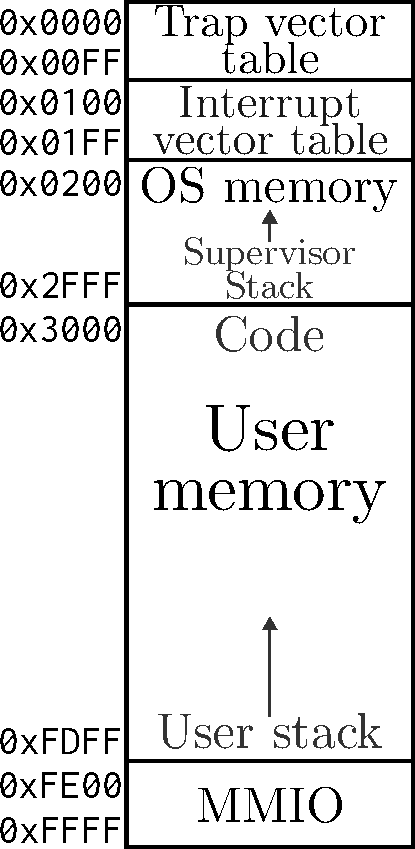
\includegraphics[width=0.33\linewidth]{figs/lc3-memory-map}

    \fi
    \ifc
    \else
        \newpage
\section*{LC-3 Datapath Control Signals}
\begin{center}
    \large
    \textit{(Use these for filling out LC-3 FSM \textbf{state transition diagrams})}
\end{center}
\raggedright
\begin{minipage}{0.25\linewidth}
\subsection*{Signals to assert:}
\Large
\begin{itemize}
    \item \textbf{\texttt{LD.MAR}}
    \item \textbf{\texttt{LD.MDR}}
    \item \textbf{\texttt{LD.IR}}
    \item \textbf{\texttt{LD.REG}}
    \item \textbf{\texttt{LD.CC}}
    \item \textbf{\texttt{GatePC}}
    \item \textbf{\texttt{GateMDR}}
    \item \textbf{\texttt{GateALU}}
    \item \textbf{\texttt{GateAddr}}
    \item \textbf{\texttt{MEM.EN}}
\end{itemize}
\end{minipage}
\rule[-10em]{0.4pt}{20em}
\hspace{1em}
\begin{minipage}{0.65\linewidth}
\subsection*{Signals with named values:}
\Large
\begin{itemize}
    \item \textbf{\texttt{PCMUX}}: \texttt{PC+1}, \texttt{BUS}, \texttt{ADDER}
    \item \textbf{\texttt{SR1MUX}}: \texttt{IR[11:9]}, \texttt{IR[8:6]}
    \item \textbf{\texttt{DRMUX}}: \texttt{IR[11:9]}, \texttt{7}
    \item \textbf{\texttt{ALUK}}: \texttt{ADD}, \texttt{AND}, \texttt{NOTA}, \texttt{PASSA}
    \item \textbf{\texttt{ADDR1MUX}}: \texttt{PC}, \texttt{BaseR}
    \item \textbf{\texttt{ADDR2MUX}}: \texttt{ZERO}, \texttt{offset6}, \texttt{PCoffset9}, \allowbreak \texttt{PCoffset11}
    \item \textbf{\texttt{MEM.RW}}: \texttt{R}, \texttt{W}
\end{itemize}
\end{minipage}

\vspace{1em}
\hrule
\centering
\section*{LC-3 Microcode Control Signal Bit Assignments}
\begin{center}
    \large
    \textit{(Use these for filling out bits in \textbf{microcode tables})}
\end{center}
\vspace{1em}
%\raggedright
\centering
\begin{minipage}{0.35\linewidth}
    \Large
    \begin{itemize}
        \item \textbf{\texttt{PCMUX}}:
            \begin{itemize}
                \item ${00}_2 \rightarrow$ \texttt{PC+1}
                \item ${01}_2 \rightarrow$ \texttt{BUS}
                \item ${10}_2 \rightarrow$ \texttt{ADDER}
            \end{itemize}
        \item \textbf{\texttt{SR1MUX}}:
            \begin{itemize}
                \item $0 \rightarrow$ \texttt{IR[11:9]}
                \item $1 \rightarrow$ \texttt{IR[8:6]}
            \end{itemize}
        \item \textbf{\texttt{DRMUX}}:
            \begin{itemize}
                \item $0 \rightarrow$ \texttt{IR[11:9]}
                \item $1 \rightarrow$ \texttt{7}
            \end{itemize}
        \item \textbf{\texttt{ALUK}}:
            \begin{itemize}
                \item ${00}_2 \rightarrow$ \texttt{ADD}
                \item ${01}_2 \rightarrow$ \texttt{AND}
                \item ${10}_2 \rightarrow$ \texttt{NOTA}
                \item ${11}_2 \rightarrow$ \texttt{PASSA}
            \end{itemize}
    \end{itemize}
\end{minipage}
%\rule[-10em]{0.4pt}{20em}
\hspace{1em}
%\hfil
\begin{minipage}{0.35\linewidth}
\Large
\begin{itemize}
    \item \textbf{\texttt{ADDR1MUX}}:
        \begin{itemize}
            \item $0 \rightarrow$ \texttt{PC}
            \item $1 \rightarrow$ \texttt{BaseR}
        \end{itemize}
    \item \textbf{\texttt{ADDR2MUX}}:
        \begin{itemize}
            \item ${00}_2 \rightarrow$ \texttt{ZERO}
            \item ${01}_2 \rightarrow$ \texttt{offset6}
            \item ${10}_2 \rightarrow$ \texttt{PCoffset9}
            \item ${11}_2 \rightarrow$ \texttt{PCoffset11}
        \end{itemize}
    \item \textbf{\texttt{MARMUX}}:
        \begin{itemize}
            \item $0 \rightarrow$ \texttt{IR[7:0]}
            \item $1 \rightarrow$ \texttt{ADDER}
        \end{itemize}
    \item \textbf{\texttt{MEM.RW}}:
        \begin{itemize}
            \item $0 \rightarrow$ \texttt{R}
            \item $1 \rightarrow$ \texttt{W}
        \end{itemize}
\end{itemize}
\end{minipage}

        \newpage
\ifio
    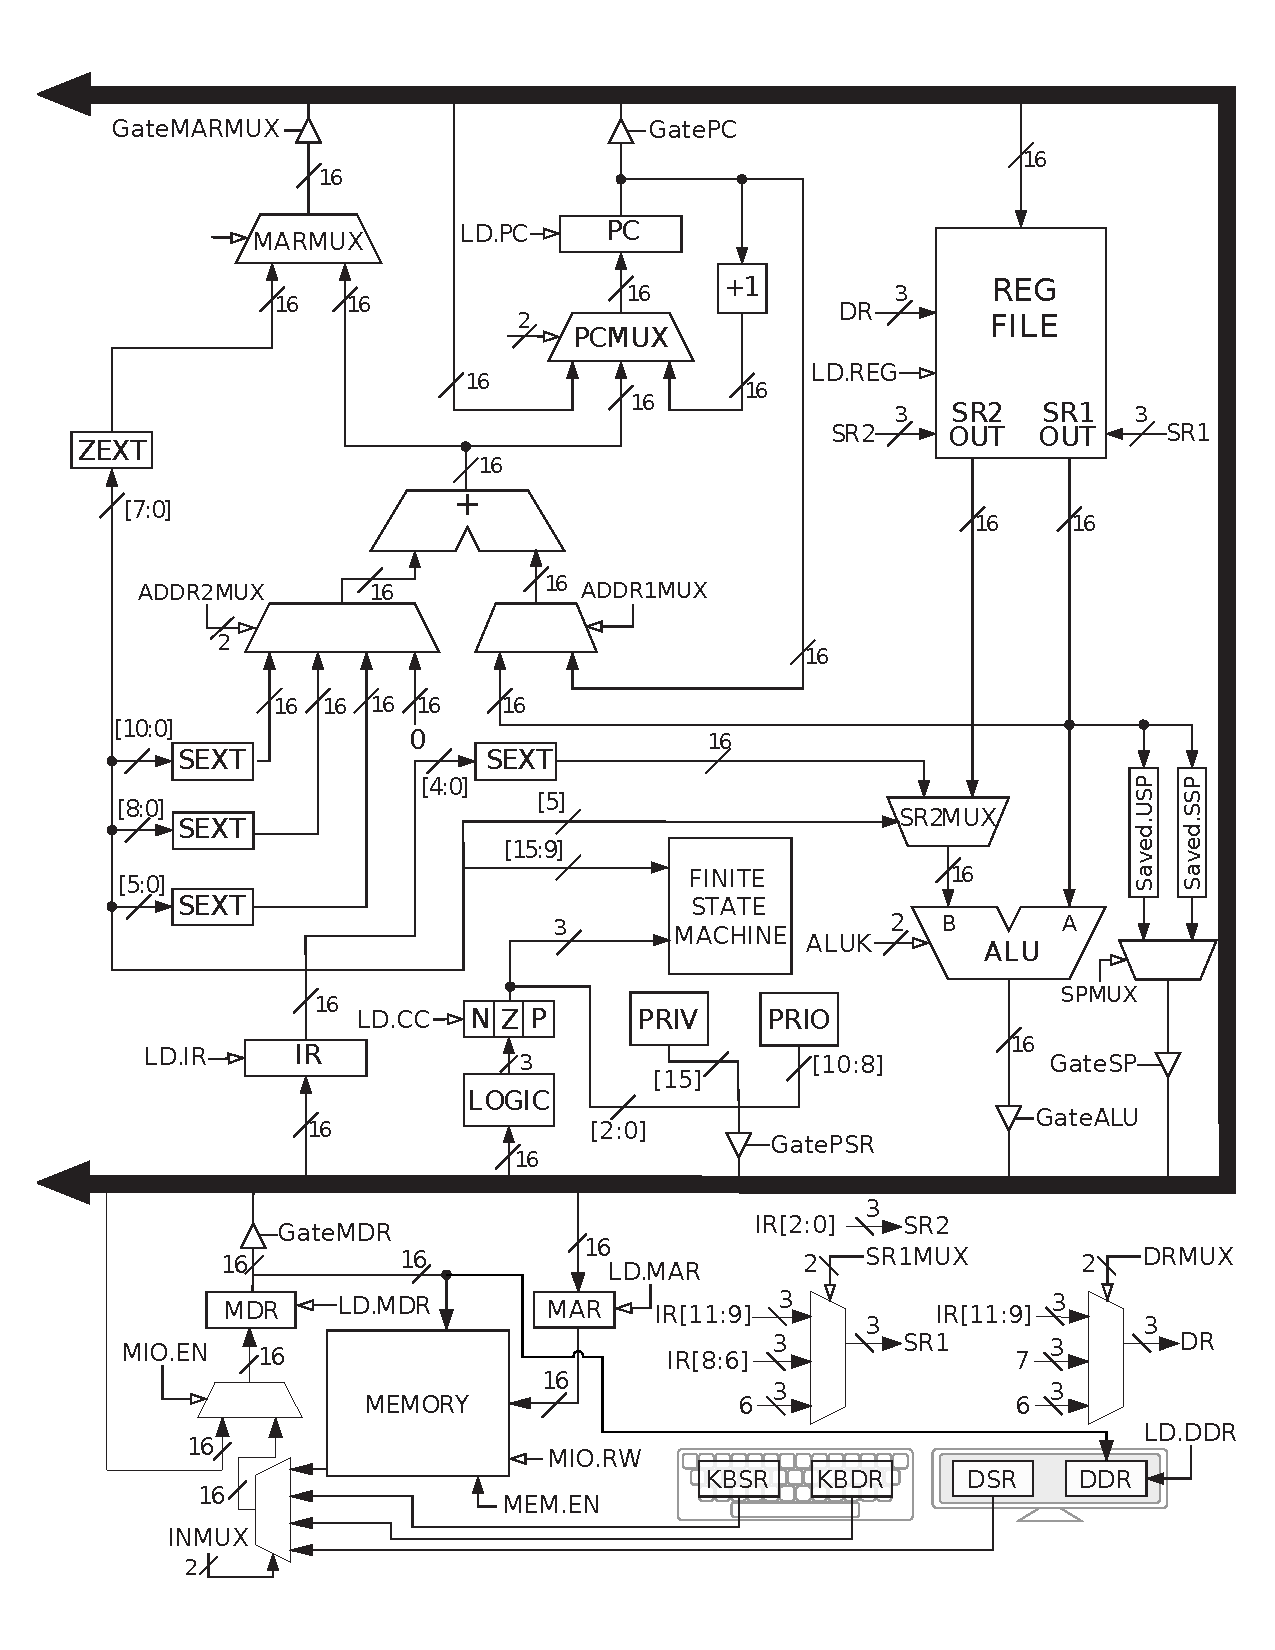
\includepdf{figs/io-letter}
\else
    
\includepdf{../pdf/11-jsr.pdf}
\fi

    \fi
\end{document}
